\subsection{\texorpdfstring{SYSTEMS OF TYPE \(\mathbf{A}_l\) (\(l \geqslant 1\))}{SYSTEMS OF TYPE A\_l (l >= 1)}}

\begin{enumerate}
\def\labelenumi{(\Roman{enumi})}
\tightlist
\item
  and (II) Let \(V\) be the hyperplane in \(E = R^{l + 1}\) with equation \(\sum_{i=1}^{l + 1} \xi_i = 0\) . Replacing \(l\) by \(l + 1\) in no. 5, we obtain a system \(R'\) of type \(B_{l + 1}\) in \(E\) with basis
\end{enumerate}

\[
\alpha_ {1} = \varepsilon_ {1} - \varepsilon_ {2}, \alpha_ {2} = \varepsilon_ {2} - \varepsilon_ {3}, \dots , \alpha_ {l} = \varepsilon_ {l} - \varepsilon_ {l + 1}. \alpha_ {l + 1} = \varepsilon_ {l + 1}.
\]

Since \(\alpha_{1},\ldots,\alpha_{l}\) generate V, \(R=R^{\prime}\cap V\) is a root system in V with basis \((\alpha_{1},\ldots,\alpha_{l})\) (§ 1, no. 7, Cor. 4 of Prop. 20). By the calculation of the scalar products in no. 5, it is immediate that R is of type \(A_{l}\) . The elements of R are the \(\varepsilon_{i}-\varepsilon_{j}\) ( \(i\neq j,1\leqslant i\leqslant l+1,1\leqslant j\leqslant l+1\) ). There are \(n=l(l+1)\) roots. The positive roots are the \(\varepsilon_{i}-\varepsilon_{j}\) where \(i<j\) .

\begin{enumerate}
\def\labelenumi{(\Roman{enumi})}
\setcounter{enumi}{2}
\item
  We have \(h = n / l = l + 1\) .
\item
  Let \(\tilde{\alpha} = \varepsilon_1 - \varepsilon_{l+1} = \alpha_1 + \alpha_2 + \cdots + \alpha_l\) , which is a root. The sum of its coordinates relative to \((\alpha_i)\) is \(l = h - 1\) . Hence \(\tilde{\alpha}\) is the highest root.
\end{enumerate}

For \(l = 1\) . \(\tilde{\alpha} = \alpha_{1}\) so \((\tilde{\alpha}|\alpha_{1}) = 2\) ; the Coxeter graph of the group \(W_{a}(R)\) is

For \(l \geqslant 2\) , \((\tilde{\alpha}|\alpha_i) = 0\) for \(0 < i < l\) and \((\tilde{\alpha}|\alpha_1) = (\tilde{\alpha}|\alpha_l) = 1\) . Hence the completed Dynkin graph is:

\pandocbounded{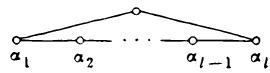
\includegraphics[keepaspectratio]{images/part002_36cfe44b.jpg}}

\begin{enumerate}
\def\labelenumi{(\Alph{enumi})}
\setcounter{enumi}{21}
\tightlist
\item
  Identifying V with its dual using the scalar product, we have \(\alpha^{\prime} = \frac{2\alpha}{(\alpha|\alpha)} = \alpha\) for all \(\alpha \in R\) , so \(R^{\prime} = R\) .
\end{enumerate}

For the form \(\Phi_{\mathbb{R}}\) , the length of the roots is \(h^{-1/2} = (l + 1)^{-1/2}\) (§ 1, no. 12); so \(\Phi_{\mathrm{R}}(x,y) = (x|y)/2(l+1)\) .

We have \(\gamma (\mathbb{R}) = (l + 1)^2\) (§ 1. no. 12, formula (20)).

\begin{enumerate}
\def\labelenumi{(\Roman{enumi})}
\setcounter{enumi}{5}
\tightlist
\item
  Let \((\omega_{i})_{1\leqslant i\leqslant l}\) be the family of fundamental weights. Put
\end{enumerate}

\[
\omega_ {i} = \sum_ {j = 1} ^ {l + 1} \xi_ {i j} \varepsilon_ {j}. \quad \text { with } \xi_ {i j} \in \mathbf {R}.
\]

The conditions \((\omega_{i}|\alpha_{j}) = \delta_{ij}\) and \(\omega_{i}\in V\) give

\[
\xi_ {i i} - \xi_ {i, i + 1} = 1, \quad \xi_ {i j} - \xi_ {i, j + 1} = 0 \text {   for   } j \neq i, \quad \sum_ {j = 1} ^ {l + 1} \xi_ {i j} = 0,
\]

which easily lead to

\[
\begin{array}{r l} \omega_ {i} & = \varepsilon_ {1} + \dots + \varepsilon_ {i} - \frac {i}{l + 1} (\varepsilon_ {1} + \dots + \varepsilon_ {l + 1}) \\ & = \frac {1}{l + 1} ((l - i + 1) (\alpha_ {1} + 2 \alpha_ {2} + \dots + (i - 1) \alpha_ {i - 1}) \\ & \quad + i ((l - i + 1) \alpha_ {i} + (l - i) \alpha_ {i + 1} + \dots + \alpha_ {l})). \end{array}
\]

\begin{enumerate}
\def\labelenumi{(\Roman{enumi})}
\setcounter{enumi}{6}
\tightlist
\item
  The sum of the positive roots is
\end{enumerate}

\[
\begin{array}{r l} 2 \rho & = l \varepsilon_ {1} + (l - 2) \varepsilon_ {2} + (l - 4) \varepsilon_ {3} + \dots - (l - 2) \varepsilon_ {l} - l \varepsilon_ {l + 1} \\ & = l \alpha_ {1} + 2 (l - 1) \alpha_ {2} + \dots + i (l - i + 1) \alpha_ {i} + \dots + l \alpha_ {l}. \end{array}
\]

\begin{enumerate}
\def\labelenumi{(\Roman{enumi})}
\setcounter{enumi}{7}
\tightlist
\item
  Introduce in \(\mathbf{E} = \mathbf{R}^{l + 1}\) the subgroup \(\mathrm{L}_0\) of no. 4. Let \(p\) be the orthogonal projection of E onto V. By § 1, no. 10, Prop. 28, we have
\end{enumerate}

\[
\mathrm{Q} (\mathrm{R}) = \mathrm{Q} \left(\mathrm{R} ^ {\prime}\right) \cap \mathrm{V} \neq \mathrm{L} _ {0} \cap \mathrm{V}, \text { and } \mathrm{P} (\mathrm{R}) = p \left(\mathrm{P} \left(\mathrm{R} ^ {\prime}\right)\right);
\]

in view of the fact that the last fundamental weight of \(R'\) is orthogonal to V, we have \(\mathrm{P}(\mathrm{R}) = p(\mathrm{Q}(\mathrm{R}')) = p(\mathrm{L}_0)\) . Thus, \(\mathrm{P}(\mathrm{R})\) is the group generated by the \(\varepsilon_i - \varepsilon_j\) and by \(p(\varepsilon_1) = \varepsilon_1 \to (l + 1)^{-1} \sum_{i=1}^{l+1} \varepsilon_i\) , so

\[
\mathrm{P} (\mathrm{R}) = \mathrm{Q} (\mathrm{R}) + \mathbf {Z} \left(\varepsilon_ {1} - (l + 1) ^ {- 1} \sum_ {i = 1} ^ {l + 1} \varepsilon_ {i}\right).
\]

Now \(l + 1\) is the smallest integer \(m > 0\) such that \(mp(\varepsilon_1) \in Q(R)\) . Thus \(P(R)/Q(R)\) is isomorphic to \(\mathbf{Z}/(l + 1)\mathbf{Z}\) and the connection index is \(l + 1\) .

\begin{enumerate}
\def\labelenumi{(\Roman{enumi})}
\setcounter{enumi}{8}
\tightlist
\item
  and (X) For any automorphism g of V, let \(\varphi(g)\) be the automorphism of E that extends g and leaves \(\varepsilon_{1} + \varepsilon_{2} + \cdots + \varepsilon_{l}\) invariant. If g is the orthogonal reflection \(s_{\varepsilon_{i} - \varepsilon_{j}}|V\) , \(\varphi(g)\) is equal to \(s_{\varepsilon_{i} - \varepsilon_{j}}\) , which interchanges \(\varepsilon_{i}\) and \(\varepsilon_{j}\) and leaves fixed the \(\varepsilon_{k}\) with k distinct from i and j. Let
\end{enumerate}

\[
X = \left\{\varepsilon_ {1}, \varepsilon_ {2}, \dots , \varepsilon_ {l + 1} \right\}.
\]

Then \(g \mapsto \varphi(g)|_{\mathbf{X}}\) is an isomorphism from \(W(\mathbf{R})\) to the symmetric group of \(\mathbf{X}\) . Thus, \(W(\mathbf{R})\) is isomorphic to the symmetric group \(\mathfrak{S}_{l+1}\) , and so is of order \((l+1)!\) .

The symmetric algebra \(\mathbf{S}(\mathrm{E})\) can be identified canonically with the algebra of polynomial functions \(\mathrm{P}(\xi_1, \xi_2, \ldots, \xi_{l+1})\) on E. Let \(\mathrm{G} = \varphi(\mathrm{W}(\mathrm{R}))\) . By the preceding paragraph, the set \(\mathbf{S}(\mathrm{E})^{\mathrm{G}}\) of elements of \(\mathbf{S}(\mathrm{E})\) invariant under G is the set of symmetric polynomials (Algebra, Chap. V, App. I), and consequently (ibid.) is the algebra generated by the functions

\[
s _ {i} ^ {\prime} = \sum_ {\tau \in \mathfrak {S} _ {l + 1}} \xi_ {\tau (1)} \xi_ {\tau (2)} \dots \xi_ {\tau (i)} \quad (1 \leqslant i \leqslant l + 1).
\]

The algebra \(\mathbf{S}(\mathrm{V})\) can be identified with the restrictions to \(\mathrm{V}\) of the polynomial functions on \(\mathrm{E}\) . If \(\mathrm{P} \in \mathbf{S}(\mathrm{E})^{\mathrm{G}}\) , the restriction of \(\mathrm{P}\) to \(\mathrm{V}\) is clearly invariant under \(\mathrm{W}(\mathrm{R})\) . Conversely, if \(\mathrm{Q} \in \mathbf{S}(\mathrm{V})^{\mathrm{W}(\mathrm{R})}\) , there exists \(\mathrm{P} \in \mathbf{S}(\mathrm{E})\) extending \(\mathrm{Q}\) ; replacing \(\mathrm{P}\) by \(((l + 1)!)^{-1} \sum_{g \in \mathrm{G}} g(\mathrm{P})\) , which has the same restriction as \(\mathrm{P}\) to \(\mathrm{V}\) . we can assume that \(\mathrm{P} \in \mathbf{S}(\mathrm{E})^{\mathrm{G}}\) . Thus, \(\mathbf{S}(\mathrm{V})^{\mathrm{W}(\mathrm{R})}\) is generated by the \(s_i = s_i'|\mathrm{V}\) . Now \(s_1 = 0\) . Moreover, the transcendence degree over \(\mathbf{R}\) of the field of fractions of \(\mathbf{S}(\mathrm{V})^{\mathrm{W}(\mathrm{R})}\) is \(l\) , so the \(s_i\) ( \(2 \leqslant i \leqslant l + 1\) ) are algebraically independent. Since the \(s_i\) are of degrees \(2, 3, \ldots, l + 1\) , the exponents of \(\mathrm{W}(\mathrm{R})\) are

\[
1, 2, 3, \dots , l.
\]

\begin{enumerate}
\def\labelenumi{(\Roman{enumi})}
\setcounter{enumi}{10}
\tightlist
\item
  For \(l = 1\) . A(R) = W(R) = Z/2Z and \(w_0 = -1\) .
\end{enumerate}

For \(l \geqslant 2\) , let \(\varepsilon \in A(R)\) be the automorphism that transforms \(\alpha_i\) to \(\alpha_{l+1-i}\) . It is clear that the automorphism induced by \(\varepsilon\) is the unique non-trivial automorphism of the Dynkin graph. The group \(A(R)/W(R)\) is isomorphic to \(Z/2Z\) . Since -1 is an element of \(A(R)\) which does not belong to \(W(R)\) by (IX) and (X), we see that \(A(R)\) is isomorphic to \(W(R) \times Z/2Z\) . We have \(w_0 = -\varepsilon\) .

\begin{enumerate}
\def\labelenumi{(\Roman{enumi})}
\setcounter{enumi}{11}
\tightlist
\item
  The group \(\mathrm{P}(\mathrm{R}^{-})/\mathrm{Q}(\mathrm{R}^{-})\) is cyclic of order \(l+1\) and acts on the completed Dynkin graph by circular permutations. If \(l\geqslant2\) , the unique non-identity element of \(\mathrm{A}(\mathrm{R})/\mathrm{W}(\mathrm{R})\) acts on \(\mathrm{P}(\mathrm{R}^{-})/\mathrm{Q}(\mathrm{R}^{-})\) by the automorphism \(x\mapsto-x\) .
\end{enumerate}

